\chapter{Methodology}
\label{methodology}

\section{Overview of the Proposed Approach}
The goal of our approach is to fulfil the objective of the thesis as described in Chapter \ref{introduction}. Specifically, \todo{continue...}

The first characteristic of our approach is that we only use unsupervised methods that do not require labeled data. 

Figure \ref{fig:worklowOverview} shows the high-level pipeline of the four main steps of our research approach.

\begin{figure}[h]
    \centering
    
\begin{tikzpicture} [
    edge/.style={-latex,shorten >=1pt, thin, color=customGrey},
    line/.style={-,shorten >=1pt, thin, color=customGrey},
    mainRectangle/.style={rectangle, draw=customBlue, align=center},
    dataCollectionCylinder/.style={cylinder, draw=customBlue, shape aspect = 0.3, align=center, shape border rotate=90}
]
    % DATA COLLECTION
    \node[mainRectangle, minimum width={40mm}, label={[label distance=2mm, align=center]{ \footnotesize 1. Data collection}}] (dataCollection) at (0, 0) {
        \begin{tikzpicture}[node distance=1cm,outer sep=0pt]
          \node[dataCollectionCylinder, minimum width={25mm}, minimum height={10mm}] (dataCylinder) {\scriptsize Log file};
        \end{tikzpicture}
    };
    
    % LOG PARSING
    \node[mainRectangle, minimum width={43mm},
    label={[label distance=2mm, align=center]{\footnotesize 2. Log parsing}}] (logParsing) at (6, 0) {
        \begin{tikzpicture}[align=center]
            \node[mainRectangle, densely dashed, minimum width={30mm}, label={[label distance=0mm, align=center]{\scriptsize Template mining}}] (templateMining) {
                \begin{tikzpicture}
                    \node[rectangle, draw=customDarkRed, align=center, solid] (rawLog) at (6, -2) {\textcolor{customDarkRed}{\tiny RAW LOG}};
                    \node[rectangle, draw=customDarkRed, align=center, solid] (eventTemplate) at (6, -4) {\textcolor{customDarkRed}{\tiny LOG EVENT}};
                    \draw[edge, solid] (rawLog) -- (eventTemplate);
                \end{tikzpicture}
            };
        \end{tikzpicture}
    };
    \draw[edge] (dataCollection) -- (logParsing);
    
    % FEATURE ENGINEERING
    \node[mainRectangle, minimum width={50mm},
    label={[label distance=2mm, align=center]{\footnotesize 3. Feature engineering}}] (featureEngineering) at (6,-6) {
        \begin{tikzpicture}[node distance=1cm,outer sep=0pt]
        % WINDOWING
            \node[mainRectangle, align=center, densely dashed, minimum width={30mm}, label={[label distance=0mm, align=center]{\scriptsize Windowing}}] (windowing) {
                \begin{tikzpicture}
                    % LOG EVENTS
                    \node[rectangle, draw=customDarkRed, fill=white, align=center, solid] (logEventWindow3) at (6.2, -3.8) {\textcolor{customDarkRed}{\tiny LOG EVENT}}; 
                    \node[rectangle, draw=customDarkRed, fill=white, align=center, solid] (logEventWindow2) at (6.1, -3.9) {\textcolor{customDarkRed}{\tiny LOG EVENT}}; 
                    \node[rectangle, draw=customDarkRed, fill=white, align=center, solid] (logEventWindow1) at (6, -4) {\textcolor{customDarkRed}{\tiny LOG EVENT}};
                    
                    % LOG SEQUENCE
                    \node[rectangle, draw=customDarkRed, align=center, solid] (logSequence) at (6, -6) {\textcolor{customDarkRed}{\tiny LOG SEQUENCE}};
                    
                    \draw[edge, solid] (logEventWindow1) -- (logSequence);
                \end{tikzpicture}
            };
            
            % FEATURE VECTOR EXTRACTION
            \node[mainRectangle, align=center, densely dashed, minimum width={30mm}, label={[label distance=0mm, align=center]{\scriptsize Feature vector extraction}}] (featureVectorExtraction) at (0,-3) {
                
                \begin{tikzpicture}
                    \node[rectangle, draw=customDarkRed, align=center, solid, minimum width={15mm}] (eventCountVector) at (0, 0) {\textcolor{customDarkRed}{\tiny EVENT COUNT}\\\textcolor{customDarkRed}{\tiny VECTOR}};
                    
                    \node[rectangle, draw=customDarkRed, align=center, solid, minimum width={15mm}] at (2, 0) (tfIdfVector) {\textcolor{customDarkRed}{\tiny TF-IDF}\\\textcolor{customDarkRed}{\tiny VECTOR}};
                \end{tikzpicture} 
            };
            
            \draw[line, solid] (windowing) -- (0, -2);
            \draw[edge, solid] (0, -2) -| (-2.3, -2) |- (-1.95, -3);
            \draw[edge, solid] (0, -2) -| (2.3, -2) |- (1.85, -3);
        \end{tikzpicture}
    };
    
    \draw[edge] (node cs:name=logParsing, anchor=east) -| (9, 0) |- (node cs:name=featureEngineering, anchor=east);
    
    \node[mainRectangle, minimum width={40mm}, label={[label distance=2mm, align=center]{ \footnotesize 4. Anomaly Detection}}] (anomalyDetection) at (0, -6) {
        % FEATURE MATRIX
        \begin{tikzpicture}
            \node[rectangle, draw=customDarkRed, align=center, solid, minimum width={30mm}] (featureMatrix) at (0, -2) {\textcolor{customDarkRed}{\tiny FEATURE MATRIX}};
            
            \draw[edge, solid] (featureMatrix) -- (0, -3);
            \draw[edge, solid] (featureMatrix) -- (-1.4, -3);
            \draw[edge, solid] (featureMatrix) -- (1.4, -3);
        
         % ML METHODS
        \node[mainRectangle, align=center, densely dashed, minimum width={30mm}, label={[label distance=0mm, align=center]{\scriptsize ML Methods}}] (mlMethods) at (0,-4) {
            \begin{tikzpicture}
                \node[rectangle, draw=customDarkBlue, align=center, solid, minimum width={10mm}] (pca) at (0, 0) {\textcolor{customDarkBlue}{\tiny PCA}};
                
                \node[rectangle, draw=customDarkBlue, align=center, solid, minimum width={13mm}] at (1.4, 0) (isolationForest) {\textcolor{customDarkBlue}{\tiny ISOLATION}\\\textcolor{customDarkBlue}{\tiny FOREST}};
                
                \node[rectangle, draw=customDarkBlue, align=center, solid, minimum width={13mm}] at (3.15, 0) (invariantMining) {\textcolor{customDarkBlue}{\tiny INVARIANT}\\\textcolor{customDarkBlue}{\tiny MINING}};
            
            \end{tikzpicture} 
        };
       \end{tikzpicture}
    };
    \draw[edge] (featureEngineering) -- (anomalyDetection);
    
    \node[rectangle, draw=customGreen, align=center, solid, minimum width={10mm}] (result) at (0, -8.4) {\textcolor{customGreen}{\small Anomalies}};
    \draw[edge] (anomalyDetection) -- (result);
    
\end{tikzpicture}


    \caption{The workflow of our anomaly detection solution.}
    \label{fig:worklowOverview}
\end{figure}

\begin{enumerate}
    \item Data Collection 
    \item Log Parsing
    \item Feature Engineering
    \item Anomaly Detection.
\end{enumerate}

Throughout this chapter, we will provide a detailed description of these steps.

\subsection{Toy Example}
To better understand the mathematical modelling and encoding that is required to apply machine learning algorithms for anomaly detection and also to provide a proof of concept, that an anomalous change in logs can indeed be detected, it is nice to have a simple toy scenario. We will simulate a chain of microservices sending traffic from one end to another.

Let's set $m$ as a number of services denoted $s_i$, which are connected in a sequential fashion: $s_0 \rightarrow s_1 \rightarrow s_2 \rightarrow ... \rightarrow s_{m-1}$. Packets are being sent from $s_1$ to $s_m$.

Over the course of $n$ epochs, we send $n$ packets labeled $p_1, p_2, p_3, ..., p_n$ to $s_1$.

At every epoch, a service $s_i$ can execute one of the following simple events: 

\begin{itemize}
    \item $\mathbf{E_1}$: Successfully sent a packet
    \item $\mathbf{E_2}$: No packet was sent
\end{itemize}

For each event, we assign a probability of that event happening. For events it holds that 

\begin{gather*}
    Pr[E_1] + Pr[E_2] = 1
\end{gather*}

and each service can have a event different probability distribution.

At every step, every service $s_i$ will log the choice of event for every existing packet denoted as $s_i: p_{j_{E_k}}$. In our simple scenario, the event $E_2:$ FAIL is an anomaly. 

We will construct a machine learning model using supervised learning, logistic regression and decision tree (unlike our actual experiments, where we use strictly only unsupervised learning methods) with the goal of finding out which service failed to send a package. We will run the simulation for $n$ epochs. The prediction $Y$ of our model is either the service that failed, or no service in case of non-anomalous execution. The training set consists of vectors, where each dimension represents a service and the value at each dimension is the event executed by that service in given epoch. 

Firstly, we created a simulation and its illustration can be found in Figure \ref{figure:simulation}. We have given the simulation the following properties: 

\begin{itemize}
    \item Number of services $m = 5$: $s_0 \rightarrow ... \rightarrow s_{4}$
    \item Number of epochs $n = 5000$
    \item Events $E_1$ and $E_2$
    \item Services $s_0, s_1, s_3, s_4$ have a $1\%$ probability of event FAIL and service $s_2$ has a $5\%$ probability of a failure event $E_2$:
    \begin{align*}
        \forall i \in \{0, 1, 3, 4\}: Pr_i[E_1] &= p_i = 0.99 \\
        i = 2: Pr_i[E_1] &= p_i = 0.95
    \end{align*}
\end{itemize}

\begin{figure}\centering
    \begin{tikzpicture}[
    serviceNode/.style={circle,draw=customDarkBlue,fill=white,thick,inner sep=0pt,minimum size=8mm, thin},
    output/.style={circle,draw=black,fill=customGreen,thick,inner sep=0pt,minimum size=8mm},
    hidden/.style={circle,draw=black,fill=customRed,thick,inner sep=0pt,minimum size=8mm},
    function/.style={rectangle,draw=black,fill=customGrey,thick,inner sep=0pt,minimum size=8mm},
    post/.style={thin, -latex, color=customGrey},
    inEdge/.style={-latex,shorten >=1pt, thin,color=customGrey!50}
    ]
		% output invisible node
		\node[draw=none] (pOut) at (9, 3) {};
		
		\node[serviceNode] (s4) at (8, 3) {\tiny $s_4$}
		edge [post] node[auto] {\textcolor{black}{\tiny $p_4$}} (pOut);
		
		\node[serviceNode, label={[label distance=0.5cm,align=center,font=\fontsize{12}{12}\selectfont]\textcolor{customDarkRed}{\tiny FAIL}\\\small $Pi[E_2]=1 - p_i$}] (s3) at (6, 3) {\tiny $s_3$}
		edge [post] node[auto] {\textcolor{black}{\tiny $p_3$}} (s4);
		
		\node[serviceNode] (s2) at (4, 3) {\tiny $s_2$}
		edge [post] node[auto] {\textcolor{black}{\tiny $p_2$}} (s3);
		
		\node[serviceNode] (s1) at (2, 3) {\tiny $s_1$}
		edge [post] node[auto] {\textcolor{black}{\tiny $p_1$}} (s2);
		
		\node[serviceNode,label={[label distance=0.5cm,align=center,font=\fontsize{12}{12}\selectfont]\textcolor{customDarkBlue}{\tiny SEND}\\\small $Pi[E_1]=p_i$}] (s0) at (0, 3){\tiny $s_0$}
		edge [post] node[auto] {\textcolor{black}{\tiny $p_0$}} (s1);
		
		% input invisible node
		\node[draw=none] (p0) at (-2, 3) {}
		edge [inEdge, densely dashed] node[auto] {\textcolor{black}{\footnotesize packet}}  (s0);
\end{tikzpicture}
	\caption{An example of simulation configuration with $5$ services, with each service having its own probability distribution of events $Pr_i$}.
	\label{figure:simulation}
\end{figure}

The simulation generates a log file with log messages printed out by the services. In Below we can see some example log message entries in the simulated log file. Packet is sent sequentially between services in increasing order. If the service $i$ fails to send the package to the next service, it logs a message \texttt{No packet was sent} and the packet does not reach any other service $j$ such that $j$ > $i$. Those services also don't record any log message. 

\begin{verbatim}
========== Starting new simulation ==========
Epoch: 0 Service 0: Successfully sent a packet
Epoch: 0 Service 1: Successfully sent a packet
Epoch: 0 Service 2: Successfully sent a packet
Epoch: 0 Service 3: Successfully sent a packet
Epoch: 0 Service 4: Successfully sent a packet
Epoch: 1 Service 0: Successfully sent a packet
Epoch: 1 Service 1: Successfully sent a packet
Epoch: 1 Service 2: No packet was sent
Epoch: 2 Service 0: Successfully sent a packet
Epoch: 2 Service 1: Successfully sent a packet
Epoch: 2 Service 2: Successfully sent a packet
Epoch: 2 Service 3: Successfully sent a packet
Epoch: 2 Service 4: Successfully sent a packet
Epoch: 3 Service 0: Successfully sent a packet
Epoch: 3 Service 1: Successfully sent a packet
Epoch: 3 Service 2: Successfully sent a packet
Epoch: 3 Service 3: Successfully sent a packet
Epoch: 3 Service 4: Successfully sent a packet
Epoch: 4 Service 0: Successfully sent a packet
Epoch: 4 Service 1: Successfully sent a packet
Epoch: 4 Service 2: Successfully sent a packet
Epoch: 4 Service 3: Successfully sent a packet
Epoch: 4 Service 4: Successfully sent a packet
Epoch: 5 Service 0: Successfully sent a packet
Epoch: 5 Service 1: Successfully sent a packet
Epoch: 5 Service 2: Successfully sent a packet
Epoch: 5 Service 3: Successfully sent a packet
Epoch: 5 Service 4: Successfully sent a packet
Epoch: 6 Service 0: Successfully sent a packet
Epoch: 6 Service 1: Successfully sent a packet
Epoch: 6 Service 2: No packet was sent
 \end{verbatim}
 
We can transform the set of log messages into a vector embedding, as can be seen in Table \ref{tab:simulation}. Each row represents one epoch and each cell contains an output of the simulation of a corresponding service, where $1$ is equivalent to event $E_1$ and $0$ is equivalent to event $E_2$. In Figure \ref{fig:simulationPlot} the number of services, that successfully received and sent a packet for each epoch is shown. As expected from the probability distribution of the events, we can see that the majority of epochs finished successfully for all of the $5$ services. Service number $2$ was assigned a higher probability of failure, which corresponds with the number $2$ of successfully executed services on y axes. 

\begin{table}[!h]
\centering
\begin{tabular}{@{}p{1.5cm}p{1.5cm}p{1.5cm}p{1.5cm}p{1.5cm}p{1.5cm}@{}}
\toprule
Epoch      & $\mathbf{s_0}$ & $\mathbf{s_1}$ & $\mathbf{s_2}$ & $\mathbf{s_3}$ & $\mathbf{s_4}$ \\ \toprule
\textbf{0} & 1             & 1             & 1             & 1             & 1             \\
\textbf{1} & 1             & 1             & 0             & 0             & 0             \\
\textbf{2} & 1             & 1             & 1             & 1             & 1             \\
\textbf{3} & 1             & 1             & 1             & 1             & 1             \\
\textbf{4}          & 1             & 1             & 1             & 1             & 1             \\
\textbf{5}          & 1             & 1             & 1             & 1             & 1             \\
\textbf{6}          & 1             & 1             & 1             & 1             & 1             \\ \bottomrule
\end{tabular}
\caption{An example of numerical embedding obtained from the first $7$ epochs of toy example simulation.}\label{tab:simulation}
\end{table}

\begin{figure}[!h]
        \centerline{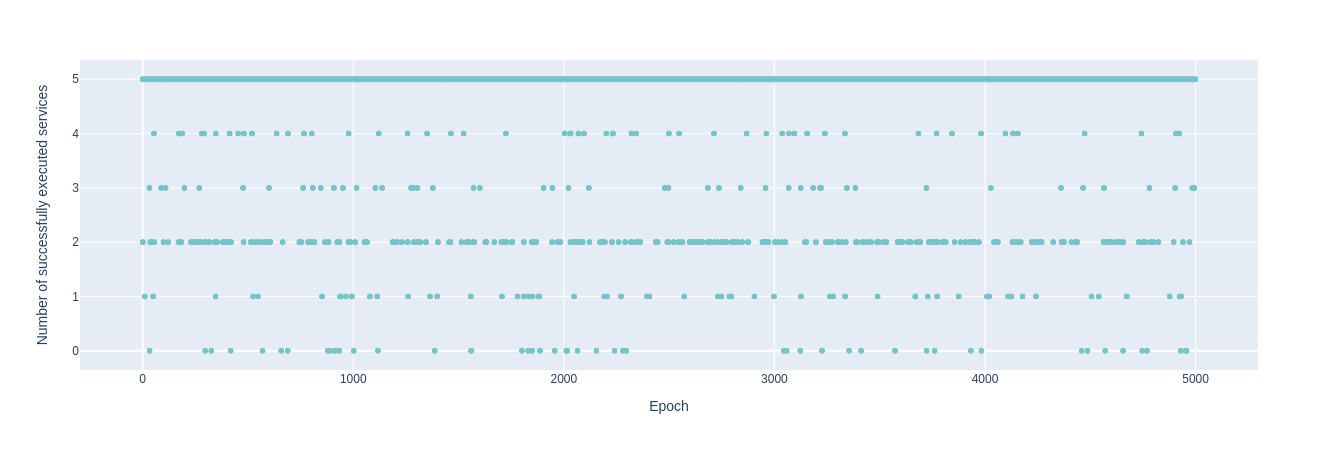
\includegraphics[scale=.35]{img/simulation-plot.png}}
        \caption{The result of running our simulation for $5000$ epochs.}
        \label{fig:simulationPlot}
\end{figure}

The obtained simulated dataset can be easily modified to generate labels. If a row is all ones, the assigned label is \texttt{no\_service}. If a row contains a zero, its label is the index of the first service that failed to send a packet. This embedding is then used as an input to create a logistic regression and random forest model. The toy example should provide a better understanding of how can a unstructured textual input be transformed into a format suitable machine learning algorithms.

\section{Data Collection}
By data collection, we understand the process of gathering log data from the observed system in such a way that the logs can be further parsed, processed, and fed to the machine learning model.
The system we study follows the microservice architectural pattern.\\
Nadareishvili et al. \cite{nadareishvili2016microservice} define a \textit{microservice} as an independently deployable component of bounded scope that supports interoperability through message-based communication. Then by \textit{microservice architecture (MSA)} they mean a style of engineering highly automated, evolvable software systems made up of capability-aligned microservices \cite{nadareishvili2016microservice}. 

Traditionally, an application performs logging by sending messages to\\
(pseudo)files \texttt{stderr} (standard error) and \texttt{stdout} (standard output). It can be combined with appending those logs also to a dedicated file with \texttt{.log} extension. Both of those practices are usually deployed by services running as containerized applications in pods. \footnote{\url{https://kubernetes.io/docs/concepts/cluster-administration/logging/}}

In microservice architecture, this approach method of logging may not be sufficient as the logs are scattered at many locations since a MSA system is usually comprised of many these applications. Also the individual services may be often replaced and contents of log files therefore removed.

Moreover, in systems that are generating big sizes and amounts of log messages, persisting logs in files that are stored in filesystem of a service pod may eventually lead to taking up all of the node's storage. 
That's why services such as \texttt{logrotate}\footnote{\url{https://linux.die.net/man/8/logrotate}} are being used. Logrotate collect logs, sends them to a different location where they can be persisted without affecting MSA system's performance and removes them from pod's node. 
This, on the other hand, means that when inspecting a pod, only the most recent (if any) logs can be found in pod's \texttt{log} file.

When it comes to SmartConnect MSA, a similar approach to the one 


\subsection{Elasticsearch}\todo{this maybe belongs to literature review?}
Elasticsearch is an open-source, distributed search engine. Gormley and Tong \cite{gormley2015elasticsearch} argue that it can be used for exploring data at unprecedented speed. It is mostly recognized for its exceptional performance on text based data. Operations such as full-text search, structured search and analysis are supported efficiently.
It can also be defined as a NoSQL database since Elasticsearch gathers JSON based \texttt{documents} of a specific \texttt{type} together and multiple \texttt{types} are organized into \texttt{indices}\footnote{\url{https://www.elastic.co/blog/what-is-an-elasticsearch-index}}. 

\subsection{Implementation}

To sum up our options for collection logs of the system:
\begin{enumerate}
    \item Downloading logs from services through \texttt{kubectl logs \${POD}} command
    \item Collecting data saved in \texttt{\${POD}:/var/log/*.log}
    \item Requesting logs from MSI's Elasticsearch server
\end{enumerate}


\section{Log Parsing}
This section describes our technique for parsing the raw and unstructured logs obtained from the analyzed system.
As pointed out in Section~\ref{log_parsing_techniques} there is many different fundamental approaches to what techniques should be used when extracting message templates from logs. 
Therefore, we developed an extra layer of abstraction over the actual parsers that makes our solution less dependent on what specific template mining algorithm is being used.

The experiments therefore work with an object \texttt{LogCategorizer} that exposes functionality to clients. To mention some of the \texttt{LogCategorizer} methods, it provides among others these ones:

\begin{itemize}
    \item \texttt{process\textunderscore log\textunderscore message(self, log\textunderscore message: str)\\ -> LogCategory}
    \item \texttt{process\textunderscore log\textunderscore messages(self, log\textunderscore messages: List[str])\\ -> List[LogCategory]}
    \item \texttt{process\textunderscore file(self, input\textunderscore file\textunderscore name: str)}
\end{itemize}

The actual reading and template creating done by these methods is carried out by an instance of \texttt{LogParser}. \texttt{LogParser} is an abstraction - an interface that is used by \texttt{LogCategorizer}. Every implementation of parser needs to fulfill this contract defined by the interface. The interface defines just the bare minimum functionality that is required from a sensible log template miner and that is a pair of methods:
\begin{itemize}
    \item \texttt{get\textunderscore all\textunderscore templates(self) -> List[str]}
    \item \texttt{process\textunderscore log\textunderscore message(self, log\textunderscore message: str) -> str}
\end{itemize}
Therefore an implementation of a log parser should be able to return all the templates that it identified by the moment the \texttt{get\textunderscore all\textunderscore templates} method is called. The other method returns a template based on the raw log message inputed.\\

Our implementation follows the adapter design pattern \cite{gamma1995design_pattern_adapter} as the aim is to convert interfaces of specific log parsing libraries that may be dramatically different in terms of the API that they expose.

This allows us to decouple the implementation of the algorithm that identifies templates from logs from our overall goal and opens the way for easy comparison with different template mining strategies.\\

\begin{figure}[!tbp]
    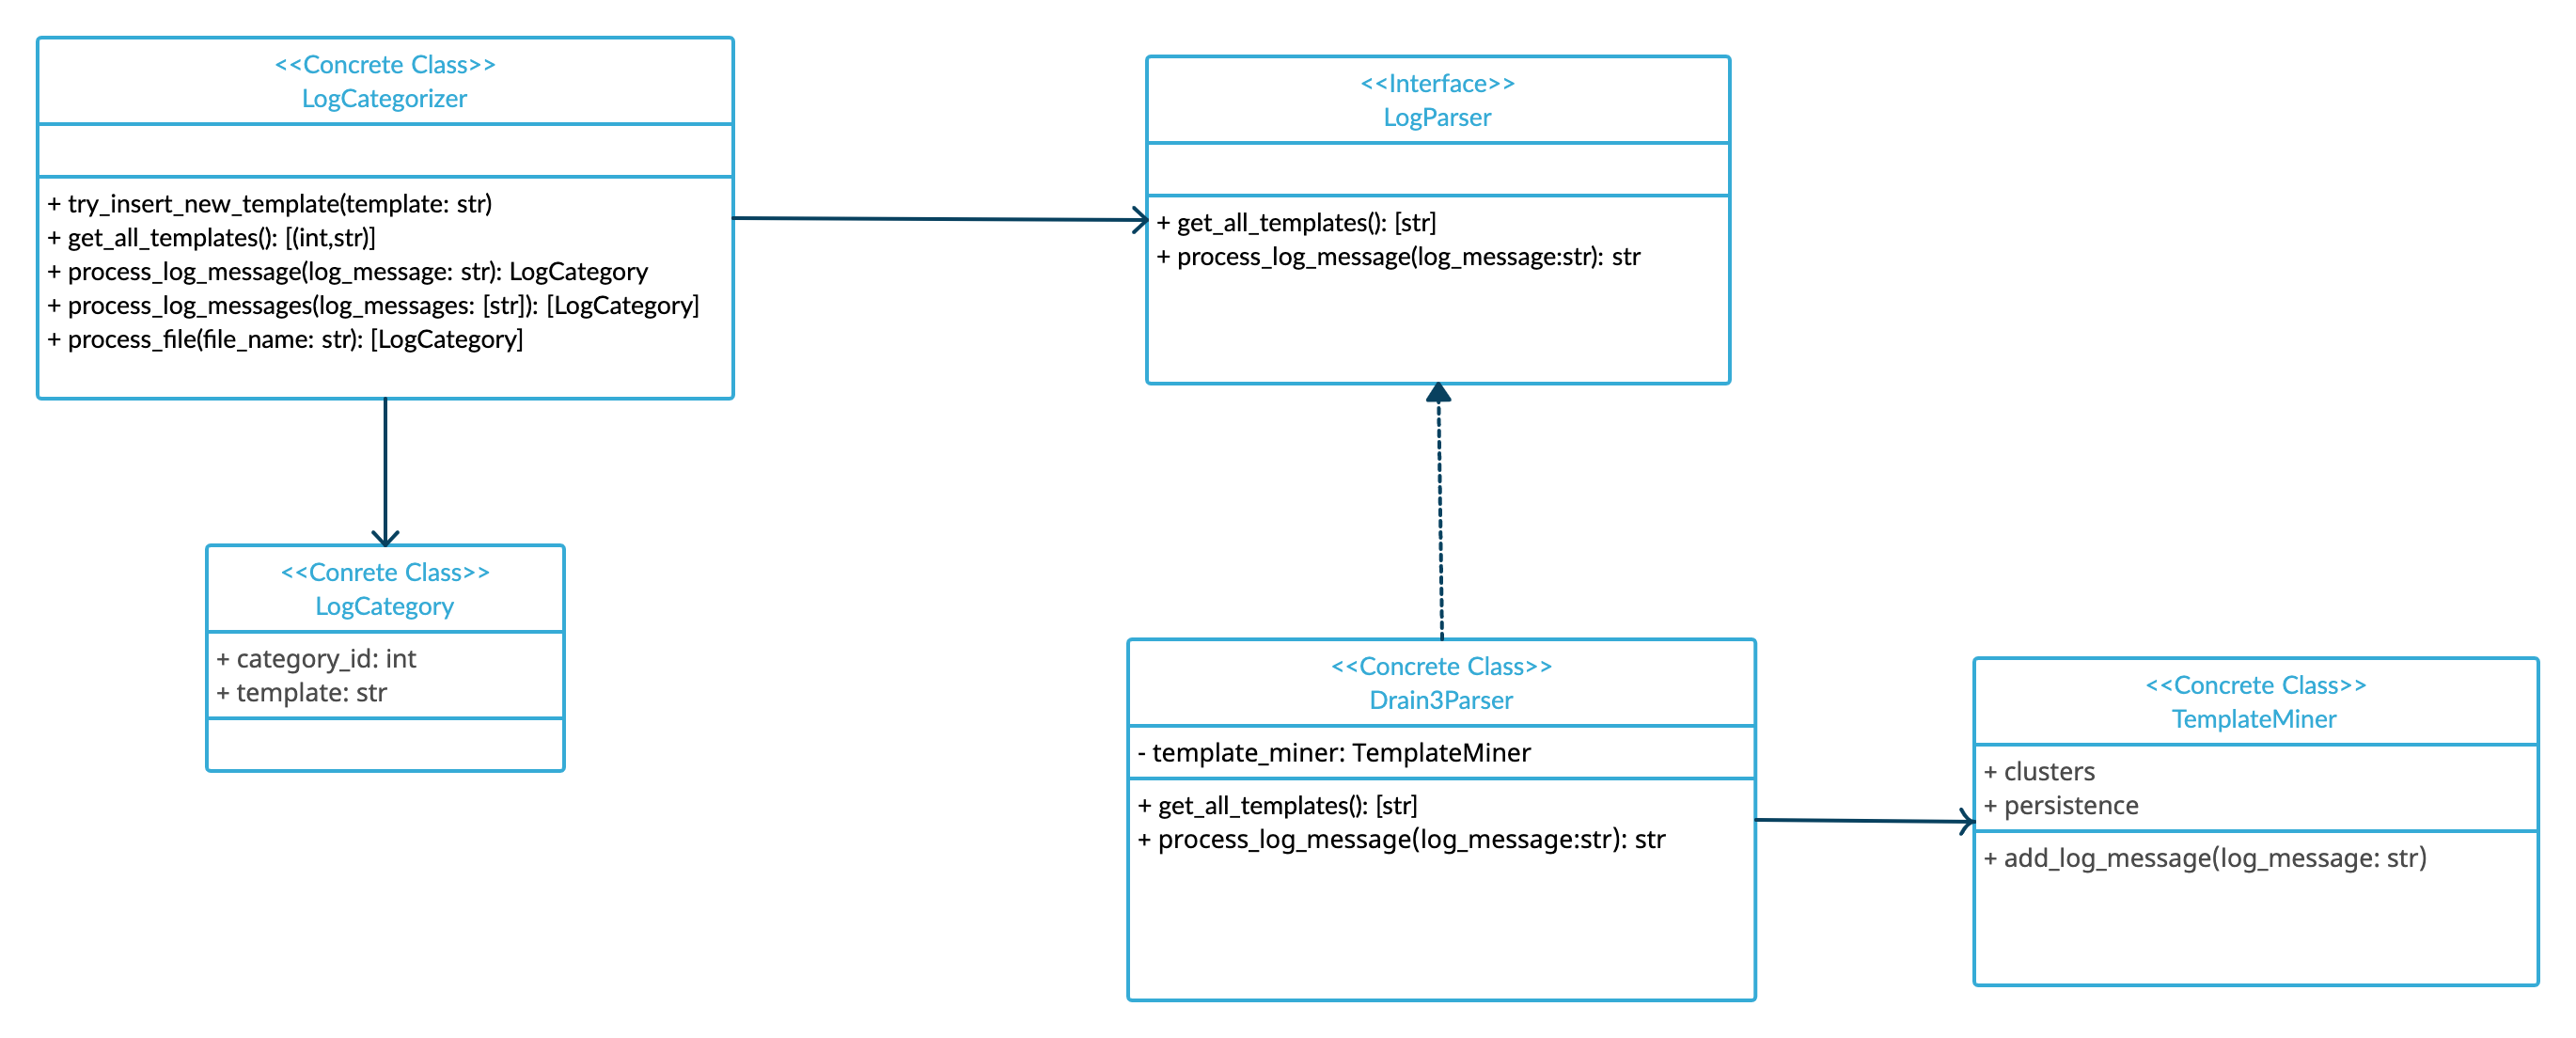
\includegraphics[width=\textwidth]{img/UML Adapter LogParser.png}		    
    \caption{Architecture for parsing classes. Adapter design pattern application: \texttt{LogParser} as the adapter, \texttt{Drain3Parser} takes on the role of concrete adaptee, \texttt{TemplateMiner} is adaptee - class defined in a different framework with incompatible interface that needs to be converted.}
	\label{fig:uml_parsers}
\end{figure}

In Section~\ref{parser_summary} we mention that our decision was to progress with the framework Drain \cite{drain2017} that performs online fixed-depth tree template mining. The actual implementation of the algorithm we used is \texttt{Drain3} by company IBM\footnote{\url{https://github.com/IBM/Drain3}}. The algorithm follows a template of 5 steps, as described in more depth in Section~\ref{fixed_depth_tree}:
\begin{enumerate}
    \item Preprocess by Domain Knowledge
    \item Search by Log Message Length
    \item Search by Precending Tokens
    \item Search by Token Similarity
    \item Update the Parse Tree
\end{enumerate}

Let's pay more attention to the first step. It provides us, users, the option to input encoded assumptions and insight on the logs that are produced by the logs.
It is rather intuitive to assume that this domain knowledge, if inserted correctly, should improve the performance and precision of the mining algorithm. An empirical study \cite{he2016} confirms this assumption.
We, however, argue that this technique that tunes the algorithm may not be the option to choose in all use cases. With our solution, we are seeking to analyze a system that is very fluid, therefore likely to change over time. This, together with the fact many developers from multiple teams and companies (taking into account also external software the software system is dependent on), it is unfeasible to maintain a single source of truth regarding domain knowledge related to logging. Conversely, we are aiming for a solution that can learn and adapt to changes as independently as possible.\\

This goal of adaptability is also reflected on the fact that we ended up choosing an online parser.
To remind a definition of an online template miner from Section~\ref{log_template_mining}, an online template miner is such a parser, that does not require to see the whole dataset to start analyzing message templates. It can run categorization on the fly while updating its internal state, which keeps acquired knowledge about the domain.\\
Drain offers the possibility to persist this internal state even between multiple runs which offers us the best of both worlds - the parser is learning patterns occurring in logs over time to improve while being able to react to new data in flexible fashion.

We have not tweaked steps 2. - 4. as the default parameters \cite{ibmdrain3} yielded results that extracted correct templates from the observed logs.

For the last step, updating the parse tree, Drain3 implementation offers the option to persist the state of the parse tree in json file format. This allows us to reuse the  domain knowledge that is acquired by the template miner across restarts of our solution.
This is an extremely useful feature, when we may assume that all of the logs are coming from the same system, we can reuse the parse tree already build in previous runs and enrich it.
Drain3 offers multiple ways of storing the snapshot of parse tree, we are using the one that saves the state into a file.

\subsection{Abstracting Logs as Events}
\todo{log data - event type distribution plot}
\todo{distribution of event types plot}


\section{Feature Engineering}
\label{section:featureEngineering}
Now that we obtained unique event type out of unstructured log message, we need to choose valuable variables, group them together and encode them into a numerical form that can be further used by the machine learning algorithms.  This process is called \textit{feature engineering} or \textit{feature extraction}. Feature extraction is the process of generating new features by doing transformations of the original feature set.  
Feature engineering step is especially important and should be able to summarize valuable information and complex relationships in the dataset, thus directly impacts accuracy of the learning model, speed of training and avoids overfitting. Log event types generated in the previous step are used as an input for feature engineering step. The output is a numerical matrix. 

\subsection{Windowing}
% https://core.ac.uk/download/pdf/196555557.pdf page 22

In time-series anomaly detection, a common concept applied in feature extraction is \textit{windowing}. 
Logs are grouped together into smaller blocks called \textit{windows}, where each window represents a sequence of logs. In some previous approaches \cite{xu2009}, they applied windowing by grouping events by the same session identifier, such that each window represents one job execution with a unique identifier. This solution is not be not applicable to our case, as we do not have a session or process id feature in our raw data set.

Log data are also non-evenly spaced time series data, as there is naturally generated a time of occurrence of each log. As a result, another intuitive and frequently used approach is to generate a set of subsequences of time series. For example, let's say we have log lines ordered by the timestamp and the length of time window is $q$. Then the log line number $1$ to log line number $q$ will be included in the same time window $1$ and encoded as the first row of the resulting feature matrix. The goal of the next anomaly detection step is to tell for each subsequence if it contains an anomaly or not. In our thesis, we use windowing based on timestamp, which is also described in the next part of the text. \todo{update if we decide to use an identifier}   

Set of time series subsequences can be generated using \textbf{sliding windows}.

Let us consider a time series $\mathbf{x} = x_1, x_2, ..., x_n$ of length $n$. We want to extract subsequences $\mathbf{x_i}$ of length $m$. In other words, we want to apply sliding windows of length $m$ and move over the time series until we reach the end of the data set. We shift the window $r$ time steps to the right in each movement. As a result, we get $p$ windows, where $p$ is defined as 
    \begin{gather*}
        p = \dfrac{n - m}{r} + 1
    \end{gather*}

and the generated windows are of form 

\begin{gather*}
    \mathbf{x_1} = x_{11}, x_{12},..., x_{1m} \\
    \mathbf{x_2} = x_{21}, x_{22},..., x_{2m} \\
    \ldots\\
    \mathbf{x_p} = x_{p1}, x_{p2},..., x_{pm} 
\end{gather*}

Size of the step $r$ is a very important parameter. Choosing $r$ to be very low, e.g. $r = 1$ such that subsequences are obtained by sliding window one step at a time, the advantage is that no anomalous sequence can be missed with this approach. However, considering the large data set that grows over time, computations of such subsequences are inefficient and time consuming. On the contrary, we can choose a high value of $r$. For example, if we set $r$ to the length of the sliding window $m$ ($r = m$), then there is no overlap between the windows. The advantage of having a lower number of generated and decreased processing time comes with a greater risk of missing anomalous subsequences. 

Another parameter to take into consideration, is the size of the sliding window $m$. The ideal size really depends on the application domain and what's the average number of subsequent log entries that can represent an anomaly. 

Thus, setting the size of step parameter $r$ and the length of sliding window $m$ is a trade-off between accuracy and processing time. A useful rule is to choose the value of $r$ proportional to the length of subsequences \cite{izakian2013}. As a result, longer subsequences have higher value of $r$ while shorter subsequences have lower value of $r$. The number of log lines included in each window can vary. 

In our thesis, instead of setting the number of log lines in each window, we consider a size of a subsequence in terms of a time-span.

\begin{figure}[!tbp] \centering {
	\begin{subfigure}[b]{1\textwidth}
        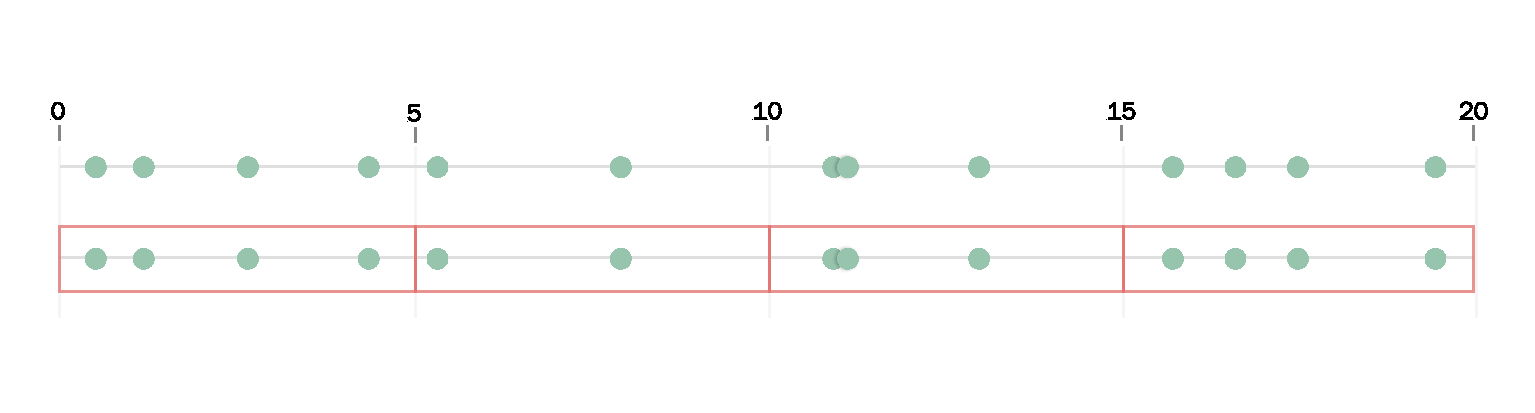
\includegraphics[width=\textwidth]{img/windowing.pdf}		    \caption{Sliding window with a fixed length of $m = 5$ and the size of the step $r = m = 5$}
		\label{fig:f1}
	\end{subfigure} \\
	\hfill
		
    \begin{subfigure}[b]{1\textwidth}
   	    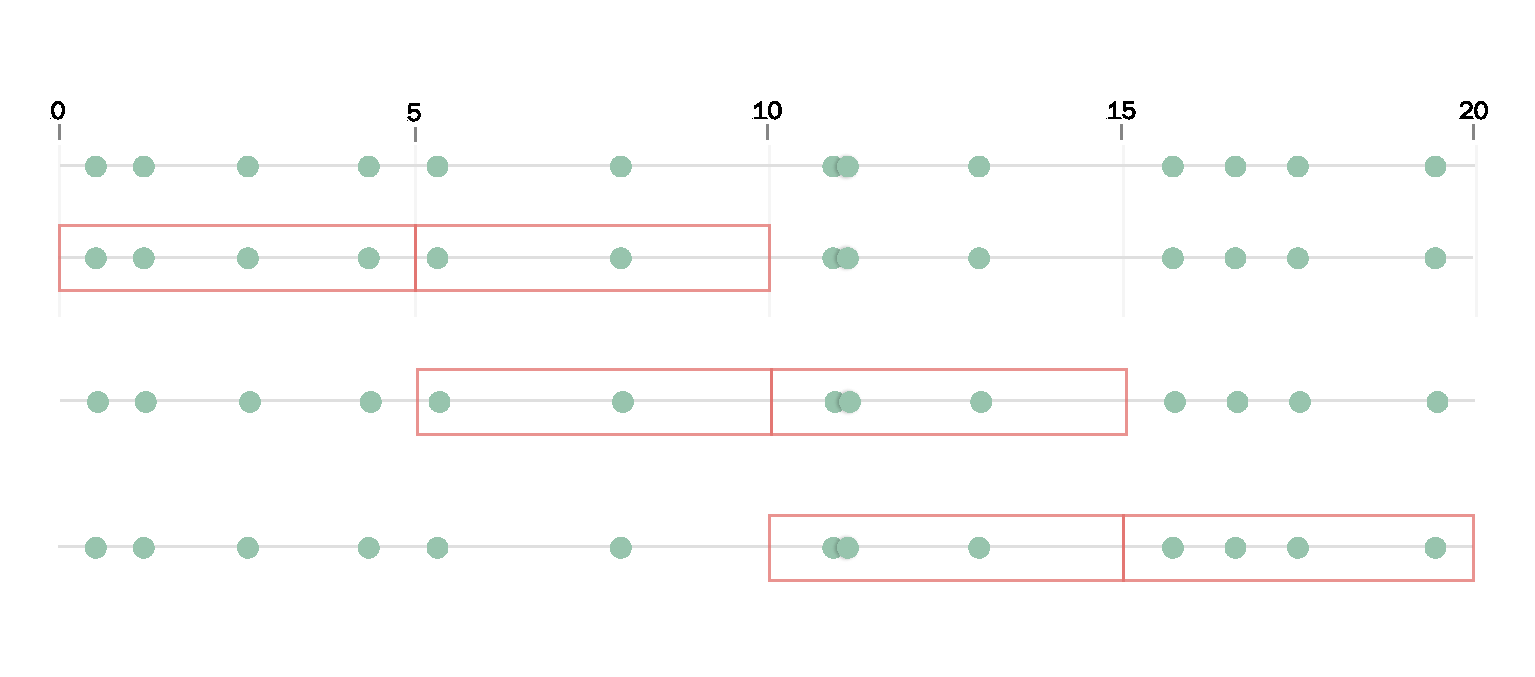
\includegraphics[width=\textwidth]{img/windowing-2.pdf}
		\caption{Sliding window with a fixed length of $m = 10$ and the size of the step $r = 5$}
	\end{subfigure}
	
	\caption{Two types of windowing with different step size $r$. (a) shows sliding windows generated without any overlap. (b) illustrates sliding window generated by stepping half of the window size at the time causing overlaps between subsequent windows.}
	\label{fig:windowing}
	}
\end{figure}

\subsection{Feature Matrix Description}
After applying the sliding window to generate the log sequences, the final step of feature extraction is to construct the feature matrix. In our thesis, we experiment with two types of feature matrices, where both representations describe a group of logs in log sequences: \textit{event count matrix} and \textit{TF-IDF weighted matrix}. Figure \ref{fig:feature-extraction} illustrates an example of a generation process of one single log sequence into a feature matrix. We assume that the logs in sequences are highly correlated.

\begin{figure}[!h] \centering {
   \begin{tikzpicture} [
    edge/.style={-latex,shorten >=1pt, thin, color=customGrey},
    line/.style={-,shorten >=1pt, thin, color=customGrey},
    mainRectangle/.style={rectangle, draw=customBlue, align=left}
]

    % RAW LOG MESSAGE SEQUENCE
    \node[mainRectangle, minimum width={110mm}, label={[label distance=2mm, align=center] { \footnotesize Raw log message sequence}}] (logSequence) at (0, 0) {
        \begin{tikzpicture}[node distance=1cm,outer sep=0pt, align=left]
            \node[draw=none] (log1) at (0, 0) {\tiny 1 \textcolor{customDarkBlue}{2020-10-04 19:15:00} Error in estabilishing TLS connection: ip: {52,240,151,125}, port: 17857\\
            \tiny 2 \textcolor{customDarkBlue}{2020-10-04 19:15:07} Start call: Service.start()\\
            \tiny 3 \textcolor{customDarkBlue}{2020-10-04 19:20:01} Received message: \#PID<0.2108.0> type: DELETED rv: 55000\\
            \tiny 4 \textcolor{customDarkBlue}{2020-10-04 19:15:07} New TLS connection attempt client\_ip: \{13,65,95,152\}, port: 26097\\
            \tiny 5 \textcolor{customDarkBlue}{2020-10-04 19:15:07} Received message: \#PID<0.2108.0> type: MODIFIED rv: 55000};
        \end{tikzpicture} 
    };
    
    % EVENT TEMPLATES
    \node[mainRectangle, minimum width={90mm}, label={[label distance=2mm] { \footnotesize Event templates}}] (eventTemplates) at (0, -5) {
        \begin{tikzpicture}[node distance=1cm,outer sep=0pt]
            \node[draw=none] (templates) at (-2, 0) {
            \tiny 1 \textcolor{customDarkRed}{Event template 1} Error in estabilishing TLS connection: ip: <*>, port: <*>\\
            \tiny 2 \textcolor{customDarkRed}{Event template 2} Start call: <*>\\
            \tiny 3 \textcolor{customDarkRed}{Event template 3} Received message: \#PID<*> type: <*> rv: <*>\\
            \tiny 4 \textcolor{customDarkRed}{Event template 4} New TLS connection attempt client\_ip: <*>, port: <*>\\
            \tiny 5 \textcolor{customDarkRed}{Event template 5} Received message: \#PID<*> type: <*> rv: <*>};
        \end{tikzpicture} 
    };
    
    \draw[edge] (logSequence) -- (0, -3.1) node [midway, fill=white] {\footnotesize \textcolor{customGreen}{log parsing}};
    
     % EVENT TEMPLATES
    \node[mainRectangle, label={[label distance=2mm] { \footnotesize Feature vectors}}] (featureVectors) at (0, -9.5) {
        \begin{tikzpicture}[node distance=1cm,outer sep=0pt]
             % ML METHODS
            \node[mainRectangle, align=center, densely dashed, minimum width={15mm}, label={[label distance=0mm, align=center]{\scriptsize Event count vector}}] (eventCountVector) at (-1, -9.5) {
                \begin{tikzpicture}[
                    cell/.style={draw, minimum width={4mm}, minimum height={4mm}, solid, thin}
                ]
                \matrix [nodes=draw] 
                {
                \node [cell] {\tiny 1}; & \node [cell] {\tiny 1};   & \node [cell] {\tiny 2}; & \node [cell] {\tiny 1}; & \node[cell]  {\tiny 0};  & \node[cell]  {\tiny 0}; & \node [cell] {\tiny 0}; & \node [cell] {\tiny 0};\\
            };
                \end{tikzpicture} 
            };
            
            \node[mainRectangle, align=center, densely dashed, minimum width={15mm}, label={[label distance=0mm, align=center]{\scriptsize TF-IDF vector}}] (tfIdfVector) at (4, -9.5) {
                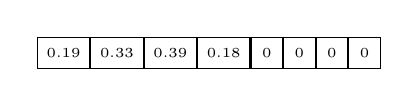
\begin{tikzpicture} [
                    cell/.style={draw, minimum width={4mm}, minimum height={4mm}, solid, thin}
                ]
                \matrix [nodes=draw]
                {
                \node [cell] {\tiny 0.19}; & \node [cell] {\tiny 0.33};   & \node [cell] {\tiny 0.39}; & \node [cell] {\tiny 0.18}; & \node[cell]  {\tiny 0};  & \node[cell]  {\tiny 0}; & \node [cell] {\tiny 0}; & \node [cell] {\tiny 0};\\
            };
                \end{tikzpicture} 
            };
        \end{tikzpicture} 
    };
    
    \draw[edge] (eventTemplates) -- (0, -8) node [midway, fill=white] {\footnotesize \textcolor{customGreen}{feature extraction}};
    

\end{tikzpicture}
   \caption{An example of encoding log sequence into two types of feature vectors: \textit{Event count vector} and \textit{TF-IDF vector}. We assume that there is $8$ event templates in the collection, thus the output vectors are also of length $8$.}
	\label{fig:feature-extraction}
	}
\end{figure}

\subsubsection*{Event Count Matrix}
A simple approach to obtain such representation is to create a event count vector for each log sequence. In other words, for each log sequence, we count the number of occurred event type identifiers and store it as a row vector of an event count matrix. The length of the vector corresponds with the number of unique event types detected in the log parsing section, and each component of the vector corresponds to one event type. The value at each position in the vector is the frequency of event types. For event types that did not occur in the log sequence, the value is zero. Thus, one row of the event count matrix represents a single log sequence. The valuable information contributing to the machine learning model behind the event count matrix is determining what is a normal count of events and what does it mean to deviate from the normal counts.

%http://essay.utwente.nl/83142/1/Ma_MA_FacultyOfEEMathematicsAndCS.pdf illustration

This way of constructing the event count matrix is known in the literature as a natural language processing (NLP) model for feature extraction called \textit{Bag-of-Words} (BoW) \cite{informationRetrieval2008}. BoW treats each log sequence as a \textit{document} and for each \textit{word} (in our case, a word is an event type) in a document, a \textit{weight} is assigned. The weight depends on the number of occurrences of the term in the document. The length of the vector corresponds with the number of unique words in the database (analogous to all parsed event types). Then the weight score is referred to as \textit{term frequency} (TF) and denoted as $tf_{t,d}$, where the subscript $t$ refers to term (event type) and $d$ refers to document (log sequence) and $f_{t,d}$ is a frequency of term $t$ in document $d$.

\begin{gather}
    tf_{t,d} = \dfrac{f_{t,d}}{\sum_{t'}f_{t', d}}
\end{gather}

In other words, $tf_{t, d}$ is the probability of occurrence of $t$ in $d$.


%https://www2.eecs.berkeley.edu/Pubs/TechRpts/2009/EECS-2009-103.pdf
\todo{Add dimensionality of the feature vector table}
\subsubsection*{TF-IDF}
Another weighting scheme wildly used in Information Retrieval is called \textit{term frequency–inverse document frequency} (TF-IDF). 

Using only the standard term frequency, we have to deal with an important issue. From the definition of term frequency, all event types are considered equally important \cite{informationRetrieval2008}. However, we would also like to know how important a term is not only in one document, but in the whole dataset. That's where another weight score, \textit{inverse document frequency} (IDF) comes to play. First, let us define \textit{document frequency} (DF). Document frequency $df_t$ is defined as the number of documents in the collection that contain the term $t$. Then the inverse document frequency $df_t$ of the term $t$ is defined as: 

\begin{gather}
    idf_t = \log{\dfrac{N}{df_t}}
    \label{formula:idf}
\end{gather}

where $N$ is the total number of documents in the collection. We can observe that if a term is rarely occurring in the collection, the $idf$ is high, and if the term is frequent, then the $idf$ is low.

By the definition, TF-IDF weighting of a term $t$ in document $d$ is a product of two quantities: the term frequency $tf_t$ and the inverse document frequency $idf_t$:

\begin{gather}
    tf\text{-}idf_{t, d} = tf_{t,d} \times idf_t
    \label{formula:tfidf}
\end{gather}

The intuition behind the components of TF-IDF weight is that the term frequency gives higher weight to terms that are frequently occurring in a single document. On the contrary, inverse document frequency gives lower score to words that are frequently occurring in the whole collection. Thus, the $tf\text{-}idf_{t, d}$ weight of the term $t$ in document $d$ is 

\begin{enumerate}
    \item higher, if the term $t$ is frequently occurring in the small number of documents
    \item lower, if the term $t$ is rarely occurring in the high number of documents or if the term $t$ is rarely occurring in the document $d$
    \item lowest, if the term $t$ occurs in all of the document in the collection
\end{enumerate}

As a result, the feature vector of the log sequence is a vector with the value of each dimension defined by \ref{formula:tfidf}.

\subsubsection*{TF-IDF example}
We will show an example of how TF-IDF is computed in our case, where we work with log sequences instead of documents and event type identifiers instead of terms. Let's assume we have a collection of log sequences and we extracted $8$ event templates from our dataset. Each log message found in log sequence is marked by its corresponding event type identifier starting from $1$ to $8$, as shown in Table \ref{tab:tfidfexample1}.

\begin{table}
\centering
\begin{tabular}{@{}C{10cm}C{10cm}@{}}
\toprule
\textbf{Log sequence ID} & \textbf{Event Types} \\ \toprule
$l_1$                       & {$[1, 4, 1, 3, 7]$}               \\
$l_2$                         & {$[3, 3, 3, 8, 4]$}               \\
$l_3$                         & {$[2, 7]$}               \\
$l_4$                         & {$[3, 3, 6, 8, 4, 6]$}               \\ \bottomrule
\end{tabular}
\caption{An example of log sequences, which comprises different amounts of log messages. Log message is represented by the event type identifier.}\label{tab:tfidfexample1}
\end{table}

In order to compute the term frequency, we find the frequencies event types in each log sequence and then normalize the frequencies to get the row vectors sum to $1$. To continue with our example set of log sequences, the TF score computation is described in Table \ref{tab:tfidfexample2}.

\begin{table}[!h] 
\begin{subtable}[b]{1\textwidth}
\centering
  \begin{tabular}{@{}ccccccccc@{}}
        \toprule
        \backslashbox{Log sequence ID}{Event type ID} & \textbf{1} & \textbf{2} & \textbf{3} & \textbf{4} & \textbf{5} & \textbf{6} & \textbf{7} & \textbf{8} \\ \midrule
        $l_1$                     & 2          & 0          & 1          & 1          & 0          & 0          & 1          & 0          \\ \midrule
        $l_2$                     & 0          & 0          & 3          & 1          & 0          & 0          & 0          & 1          \\ \midrule
        $l_3$                     & 0          & 1          & 0          & 0          & 0          & 0          & 1          & 0          \\ \midrule
        $l_4$                     & 0          & 0          & 2          & 1          & 0          & 2          & 0          & 1          \\ \bottomrule
        \end{tabular}
        
        \caption{Computation of the frequency $f_{t,d}$ of term $t$ in document $d$.}
    \end{subtable} \\
	\hfill
	\\
    \begin{subtable}[b]{1\textwidth}
    \centering
      \resizebox{\textwidth}{!}{\begin{tabular}{@{}ccccccccc@{}}
        \toprule
        \backslashbox{Log sequence ID}{Event type ID} & \textbf{1} & \textbf{2} & \textbf{3} & \textbf{4} & \textbf{5} & \textbf{6} & \textbf{7} & \textbf{8} \\ \midrule
        $l_1$                     & 2/5          & 0          & 1/5          & 1/5          & 0          & 0          & 1/5          & 0          \\ \midrule
        $l_2$                     & 0          & 0          & 3/5          & 1/5          & 0          & 0          & 0          & 1/5          \\ \midrule
        $l_3$                    & 0          & 1/2          & 0          & 0          & 0          & 0          & 1/2          & 0          \\ \midrule
        $l_4$                     & 0          & 0          & 1/3          & 1/6          & 0          & 1/3          & 0          & 1/6          \\ \bottomrule
        \end{tabular}}
        \caption{Computation of the TF score $tf_{t,d} = \dfrac{f_{t,d}}{\sum_{t'}f_{t', d}}$.}
    \end{subtable}%
    \caption{Computation of the TF score.}
	\label{tab:tfidfexample2}
\end{table}

To compute the IDF, we first calculate the document frequency $df_t$ of each term and use the formula \ref{formula:idf} to obtain the inverse document frequencies. 

\begin{table}[!h] 
\begin{subtable}[b]{1\textwidth}
\centering
  \begin{tabular}{@{}ccccccccc@{}}
        \toprule
        \backslashbox{Log sequence ID}{Event type ID} & \textbf{1} & \textbf{2} & \textbf{3} & \textbf{4} & \textbf{5} & \textbf{6} & \textbf{7} & \textbf{8} \\ \midrule
        \textbf{$l_1$}                     & 2          & 0          & 1          & 1          & 0          & 0          & 1          & 0          \\ \midrule
        \textbf{$l_2$}                     & 0          & 0          & 3          & 1          & 0          & 0          & 0          & 1          \\ \midrule
        \textbf{$l_3$}                     & 0          & 1          & 0          & 0          & 0          & 0          & 1          & 0          \\ \midrule
        \textbf{$l_4$}                     & 0          & 0          & 2          & 1          & 0          & 2          & 0          & 1 \\ \midrule
        $\mathbf{n_t}$                  & 1          & 1          & 3          & 3          & 0          & 1          & 2          & 2         
        \\ \bottomrule
        \end{tabular}
        
        \caption{Computation of the document frequency $df_{t}$ of term $t$.}
    \end{subtable} \\
	\hfill
	\\
    \begin{subtable}[b]{1\textwidth}
    \centering
      \resizebox{\textwidth}{!}{\begin{tabular}{@{}ccccccccc@{}}
        \toprule
        \backslashbox{Log sequence ID}{Event type ID} & \textbf{1} & \textbf{2} & \textbf{3} & \textbf{4} & \textbf{5} & \textbf{6} & \textbf{7} & \textbf{8} \\ \midrule
        \textbf{$l_1$}                     & 0.602          & 0,602          & 0.125          & 0.125          & 0          & 0.602          & 0.301          & 0.301         \\ \bottomrule
        \end{tabular}}
        \caption{Computation of the IDF score $idf_t = \log{\dfrac{N}{df_t}}$. In our example, $N=4$ as there are $4$ log sequences in the collection. For instance, IDF weight of the event type $1$ is calculated as $idf_1 = \log{\dfrac{4}{1}} = 0,602$.}
    \end{subtable}%
    \caption{Computation of the IDF score.}
	\label{tab:tfidfexample3}
\end{table}

The final step is calculating the product $TF \times IDF$ and the values are shown in Table \ref{tab:tfidfexample4}.

\begin{table}[!h]
    \centering
    \resizebox{\textwidth}{!}{\begin{tabular}{@{}ccccccccc@{}}
        \toprule
        \backslashbox{Log sequence ID}{Event type ID} & \textbf{1} & \textbf{2} & \textbf{3} & \textbf{4} & \textbf{5} & \textbf{6} & \textbf{7} & \textbf{8} \\ \midrule
        \textbf{$l_1$}                     & 0.2408          & 0          & 0.025          & 0.025          & 0          & 0          & 0.0602          & 0          \\ \midrule
        \textbf{$l_2$}                     & 0          & 0          & 0.075          & 0.025          & 0          & 0          & 0          & 0.0602          \\ \midrule
        \textbf{$l_3$}                     & 0          & 0.301          & 0          & 0          & 0          & 0          & 0.1501          & 0          \\ \midrule
        \textbf{$l_4$}                     & 0          & 0          & 0.042          & 0.021          & 0          & 0.201          & 0          & 0.05
        \\ \bottomrule
        \end{tabular}}
    \caption{TF and IDF scores from the example are multiplied to obtain TF-IDF}.
    \label{tab:tfidfexample4}
\end{table}

We assume that by using TF-IDF weighting, we will provide an extra information about the event type distribution not only in terms of log sequences, but also in the whole data set, that could potentially increase ML model's performance. 

\section{Anomaly detection}
% Describe the implementation of algorithms that we use (Logpai)

After creating the weighted feature matrix \todo{finish}
For our experiments, we are using an open-source machine learning toolkit \textit{Loglizer}. 

\subsection{Loglizer}

Loglizer is an open-source machine learning based log analysis toolkit for automated anomaly detection written in Python \cite{he2016}. Loglizer was developed for automated anomaly detection as a part of LogPAI \footnote{\url{http://www.logpai.com}}, which is collection of AI-based log analytics solutions. these log analysis tools have been used by industrial teams in Microsoft and Huawei. It includes three supervised anomaly detection models (\textit{Logistic Regression, Decision Tree, Support Vector Machine}) and six unsupervised anomaly detection models (\textit{Local Outlier Factor, One-Class SVM, Isolation Forest, Principal Component Analysis, Invariants Mining, Clustering}). At the time of writing this thesis, another two unsupervised models were in the development (\textit{DeepLog, AutoEncoder}). \\

We decided to leverage a third-party toolkit for several reason. Firstly, as the algorithms we are using in our experiments have been already implemented, there is no need to completely reinvent the wheel and write the implementation ourselves. This way we can avoid a time consuming process and rather focus on the main intention of our research - to investigate if applying various anomaly detection techniques on a real-life dataset can lead to successful results \todo{redefine}.

Another benefit is that the Loglizer anomaly detectors are working with log sequences. This means that each of the models is trained on a set of log sequences, and the output of the detector classifies whether a single log sequence is an anomaly or not. As described in Section \ref{section:featureEngineering}, we use windowing for generating the log sequences, which makes the Loglizer toolkit a great fit in our research context. Specifically, three \todo{update if using more tools} tools were used in our research: Invariants Mining, Isolation Forest and PCA. The underlying algorithms behind these tools are present in Section \ref{section:anomalyDetectionLiteratureReview}.

Implemented anomaly detection methods are evaluated on a public dataset, HDFS. Logs in HDFS dataset were collected from Amazon EC2 platform and contain $11\,175\,629$ entries \cite{xu2009}. Loglizer provides benchmarking results on both supervised and unsupervised methods separately using this dataset, which can be found in Table \ref{table:loglizer}. Evaluation metrics are explained in Section \todo{add ref to our metrics section}. Benchmarking gives a better idea of the expected performance of the anomaly detection methods we are planning to use in our work. 

Last but not least, Loglizer makes it easier to reproduce our experiments, as the code is open-source.

% Please add the following required packages to your document preamble:
% \usepackage{booktabs}
\begin{table}[h]
\centering
\begin{tabular}{@{}cccc@{}}
\toprule
\multicolumn{4}{c}{\textbf{HDFS}} \\ 
\textbf{Model}    & \textbf{Precision} & \textbf{Recall} & \textbf{F1} \\  \toprule \midrule
\multicolumn{4}{c}{\textit{Supervised Methods}}                        \\ \midrule
LR                & 0.955              & 0.911           & 0.933       \\
Decision Tree     & 0.998              & 0.998           & 0.998       \\
SVM               & 0.959              & 0.970           & 0.965       \\ \midrule
\multicolumn{4}{c}{\textit{Unsupervised Methods}}                      \\ \midrule
LOF      & 0.967              & 0.561           & 0.710       \\
One-Class SVM     & 0.995              & 0.222           & 0.363       \\
Isolation Forest  & 0.830              & 0.776           & 0.802       \\
PCA               & 0.975              & 0.635           & 0.769       \\
Invariants Mining & 0.888              & 0.945           & 0.915       \\
Clustering        & 1.000              & 0.720           & 0.837       \\ \bottomrule
\end{tabular}
\caption{Benchmarking results of three supervised and six unsupervised anomaly detection methods on HDFS dataset \cite{he2016}}.
\label{table:loglizer}
\end{table}

% Describe the metrics we use to evsluate results - check thesis ptrick konstjens

